\documentclass[11pt]{article}

\usepackage[margin=1in]{geometry}
\usepackage[T1]{fontenc}
\usepackage[utf8]{inputenc}
\usepackage{lmodern}
\usepackage{hyperref}
\usepackage{setspace}
\usepackage{tabularx}
\usepackage{graphicx}
\usepackage{ragged2e}

\newcolumntype{Y}{>{\RaggedRight\arraybackslash}X}

\hypersetup{
  pdftitle={The Construction of Living Robots: Transcription Draft},
  pdfauthor={Edmund C. Berkeley; transcription draft prepared in repository},
  pdfsubject={Transcription of a 1952 Berkeley robotics source},
  pdfkeywords={Edmund C. Berkeley, living robots, transcription, robotics}
}

\title{\emph{The Construction of Living Robots}\\\large Transcription Draft}
\author{Original work by Edmund C. Berkeley}
\date{Prepared from the 1952 source on August 5, 2026}

\begin{document}

\maketitle

\section*{Editorial Note}

This document is a cleaned transcription draft of Edmund C. Berkeley's
\emph{The Construction of Living Robots}. It is based on direct reading of the
scanned source pages, with OCR used only as a secondary aid. Spelling and
punctuation have been regularized only where the scan is clear enough to
support a confident reading.

This edition now includes the title page, introduction, contents page, all of
Part I, the main prose framework of Part II, and the full concluding section of
Part III. The most diagram-dense pages of Part II are preserved as image plates
inside the document so that Berkeley's circuit and program figures remain
available while fine-grained figure labeling and caption transcription
continues.

\section*{Title Page}

\begin{center}
\Large THE CONSTRUCTION OF LIVING ROBOTS

\normalsize
\vspace{1em}
by

Edmund C. Berkeley

\vspace{1em}
Copyright, 1952, by Edmund C. Berkeley

\vspace{1em}
First edition, published June, 1952, by Edmund C. Berkeley and Associates,\\
36 West 11 St., New York 11, N.Y.
\end{center}

\clearpage

\section*{Introduction}

The purpose of this report is to discuss the properties of robots and the
properties of living beings, and to outline how to construct robots made out of
hardware which will have the essential behavior of living beings. Part II of
the report outlines the circuits by means of which behavior can be programmed
in robots.

We do not expect that all readers will agree with the views set forth in this
report. Some will agree with the Encyclopaedia Britannica, and will say that
life is the activity peculiar to protoplasm, and therefore something made of
hardware, no matter how wonderful or lifelike its properties may be, will never
live. But we are convinced that, with the great current development of robots
and automatic computing machinery, it is important and worthwhile to bring up
and discuss the subject of living robots.

We hope this discussion, and the circuits here given, will encourage other
investigators and experimenters to try to build living robots, as we are
seeking to do; and we shall be glad to try to help anybody to the extent that
we can.

\clearpage

\section*{Contents}

\begin{center}
CONTENTS
\end{center}

\subsection*{Part I --- Discussion}

\begin{tabular*}{\textwidth}{@{\extracolsep{\fill}} r l r @{}}
1. & The Nature of Robots & 1--2 \\
2. & The Versatility of Robots & 2 \\
3. & The Nature of Life & 3--4 \\
4. & The Essential Properties of Life & 4--5 \\
5. & Robot Life & 5--6 \\
6. & Choices in Constructing Robot Life & 6 \\
7. & Robot Self-Preservation & 6--7 \\
8. & Robot Self-Maintenance & 7--8 \\
9. & Robot Reproduction & 8--9 \\
\end{tabular*}

\subsection*{Part II --- Outline for Constructing Robot Life}

\begin{tabular*}{\textwidth}{@{\extracolsep{\fill}} r l r @{}}
1. & Robot Life Species No.\ 1 & 10--11 \\
2. & Behavior & 11 \\
3. & Schematic Diagrams for the Counter-Part Robots & 11--13 \\
4. & Schematic Diagrams for the Robots & 14--19 \\
\end{tabular*}

\subsection*{Part III --- Practical Conclusions}

\begin{center}
19
\end{center}

\clearpage

\section*{Part I --- Discussion}

\subsection*{1. The Nature of Robots}

One after another the barriers to the construction of living robots are
breaking down. It would seem reasonable to expect that before a dozen more
years go by, automatic machines (i.e., robots) that possess the essential
properties of life will be ``in existence'' --- or should we say, ``alive''?
Certainly much more than half the distance to the construction of living robots
has been travelled.

Now these statements are by no means evident on their face. So let us take a
close look at the definitions, the facts, and the prospects. And the first
definition we need to pin down is robot. What is a robot?

The word ``robot'' comes from a Czech word meaning ``compulsory service.'' The
root ``robot-'' in the Slavic languages means ``work.'' And a robot is
basically a machine that is able to work by itself, an automaton.

In this sense, a clock would be a robot, and so would be an automatic screw
machine, --- which is able to perform six operations automatically one after
another on continuous metal bar stock fed through it; and so would be a traffic
light that changes from green to red and back to green again depending on
measured time only and without any regard for the particular traffic conditions
at the time.

But all these machines have just one program, which they carry out over and
over. And in the way that we think of robots these days, we require them to be
a little more versatile if they are to be called proper robots. To be a proper
robot, the machine should have at least two programs, and be able to change
from one program to some other depending on conditions in its environment. The
traffic light which responds to motor cars rolling over a pressure plate in the
road is a proper robot.

In fact, if we take a good close look at a robot of today, a proper robot, we
can come to the conclusion that it is an automatic machine with sensing organs,
thinking organs, and acting organs. It is a machine that can adapt itself to
some extent to its environment, doing different things depending on different
conditions.

\subsection*{2. The Versatility of Robots}

At work in the world today, and all of them slaves in the service of men, are
probably hundreds of species of robots, and millions of individual robots.

Almost any kind of scientific instrument can be used for the detection of
information. These instruments can become the sensing organs for robots.

Almost any kind of machine --- lathe, shovel, valve, motor, wheel, drill,
screw, or other device --- can be used for making changes in the physical
world. All of them can become the acting organs for robots.

A variety of different devices can be used for transmitting information between
the different parts of a robot: compressed air through pipes, electric currents
along wires, mechanical parts in motion, cables running through pulleys, etc.
These become the nerves and muscles of robots.

A large variety of devices may be used for reasonable operations on
information: electronic tubes, relays, cams, compressed air, feelers, latches
etc. These become the thinking organs of robots. In fact, some mechanical or
electrical robots --- like the automatic dial telephone central office with
subscriber stations, or the giant automatic electronic digital computers ---
display the development of hardware thinking organs to a prodigious extent.

But how close is a collection of these devices, integrated together into a
robot, to ``living''? What is ``living''?

\subsection*{3. The Nature of Life}

Have you ever in your imagination walked on the surface of Mars, and wondered
how you would tell if some THING you saw there were ``living'', or not? A
short tour on Mars will help us see what properties an Earth robot should have
in order that it should be called living. In some cases, while you were
walking on Mars, it might be easy to tell that some THING was alive. If the
THING could apparently detect your presence, and either move away from you,
apparently to avoid you, or move toward you, apparently to attack you, you
would at once jump to the conclusion that the THING was alive.

On Mars, you might be right. On Earth, robots of this general nature, which no
one claims are living, have already been made.

One of them is Squee, the Robot Squirrel, made in 1951 by the writer and his
associates and described in \emph{Radio-Electronics}, Dec. 1951 and
\emph{Popular Science}, July 1952. Squee is about 21 inches long, 12 inches
high, and 8 inches wide, and weighs about 16 pounds. It rolls over the floor,
hunts for a ``nut'' (a golf ball), picks it up in its ``hands'' (a metal scoop
in two halves), takes it over to its ``nest'' (a metal plate), there leaves
it, and then starts hunting for more nuts. Squee has four sensing organs: two
``eyes'' --- photocells; a ``tongue'' --- a switch; a ``foot'' with two
``toes'' --- two probes. Squee has three acting organs: a driving wheel, a
steering gear, and a scoop for ``hands''. And finally, Squee has a small brain,
of a dozen relays and tubes. But in spite of this active behavior, and more
than canine docility, no one says that Squee is alive.

But how about the difficult cases, in your tour on Mars, when the ordinary
clues that Earth beings use simply could not be relied on?

In regard to shape and structure, for example, the Mars THING would not have to
be constructed with any resemblance to either an animal or a plant of the
Earth. In fact, in view of our present knowledge, it seems unnecessary and
unlikely that the THING could be made of the same chemicals in the same
proportion as Earth protoplasm. In fact, the oxygen-less atmosphere and low
temperatures of Mars would make Earth protoplasm distinctly uncomfortable.

Even on Earth, the shape and structure problem may be far from simple. One and
the same living entity may be first an egg, then a caterpillar, then a
chrysalis, then a butterfly. Some sea animals may have more than nine larval or
nymphal metamorphoses, i.e., similar changes from infant to adult state.

In regard to size of the individual, the Mars THING would not have to have any
given or stated size, in advance of observations made on Mars. On Earth the
smallest individuals appear to be particles of a virus, about one hundred
thousandth of an inch in diameter. The largest animal is either the whale,
length 45 or 50 feet, or the fossil dinosaur, called Gigantosaurus, whose foot
print was about four feet in diameter, and whose length may have been as much
as sixty feet. The largest plant is the sequoia or redwood, which, trunk and
root together, may be over 500 feet in length.

In regard to speed of living, the speed with which the Mars THING lived could
be quite unrelated to the speed of living of animals or plants on Earth. Even
on Earth, the range of speed of living is great. Gnats do not hesitate to fly
when raindrops are falling; presumably their nervous system has no trouble
dodging raindrops in a time of the order of a hundredth or a thousandth of a
second. And the normal tempo for a response of a human being is to be about
1/5 to 1/10 of a second. At the other end of the scale, apparently, is a lotus
seed: In a Washington greenhouse, scientists have recently sprouted two lotus
seeds taken from a Manchurian fossil peat deposit, where they have apparently
rested dormant in their tough hard seed cases for at least a thousand years and
perhaps five thousand.

In regard to environment, the Mars THING could have a narrow or broad one. On
Earth, we have found so far upwards of three million species of living things;
their environment ranges from broad to narrow. Some species are relatively
independent and are at home in the air, on land, on sea, and some of the time
in the sea, like gulls. Other species have an intensely narrow environment,
like a kind of mushroom cultivated for food by certain ants in their anthills,
and growing nowhere else.

In fact, the more we think over the variations among living things on Earth,
the more difficult we can imagine the problem to be of recognizing living
things on Mars, especially if there were only a few species, minute, slow
moving, in narrow environments, with few enemies, and very limited adaptations.

\subsection*{4. The Essential Properties of Life}

What, then, are the properties of life? When do we consider that a thing is
living?

There is no easy answer that covers all the extreme cases that we know about on
Earth. Even supposing we could arrive at a definition that applied to Earth
life, it still might not fit Martian life. But we can make a short list of
apparently essential properties that would be sufficient on Mars as well as
Earth for a thing to be ``living''. We cannot claim that these properties are
all necessary, for there are many living things that do not have one or more of
these properties.

It is I think reasonable to say that if a thing has the following properties,
then it is living:

\begin{enumerate}
\item \textbf{Self.} It has a persisting, separate, individuality or entity. It
consists of matter. It has a center. In other words, it has a self.
\item \textbf{Sensation and Response.} At some stages of its existence, it has
the capacity to sense different changes in its ordinary environment, and make
different responses to them.
\item \textbf{Death.} If it is forcibly divided through its center, it loses
its individuality and all its capacity for sensations and response. In other
words, it dies.
\item \textbf{Self-Preservation.} Its ordinary responses to its ordinary
environment tend to avoid death.
\item \textbf{Self-Maintenance.} At some stages of its existence, it has the
capacity to take stuff out of its ordinary environment and use it for
maintaining and repairing its self.
\item \textbf{Reproduction.} At some stage of its existence, it has the
capacity, in its ordinary environment, of making or constructing other complete
things like itself and having the same six properties as itself.
\end{enumerate}

There are two properties left out of this list which deserve some discussion.
The first one is Sex. We are all familiar with a great many species of Earth
life in which individuals (in whole or in part) occur in two varieties, male
and female, with familiar properties for most species. Some people may be
inclined to say that sex is an essential property of life.

Actually, in plants, separate male and female flowers can be found on the same
plant, as in cucumber vines. Or male and female organs, stamens and pistils,
can be found right next to each other in the same flower, as in lilies. In
fact, in some flowers, cross-fertilization for seeds is impossible, as in the
bottle gentian which never opens its buds. In a few animals, such as aphids,
many generations can take place involving only females.

But there are species of living things on Earth, such as amoebas, bacteria, and
viruses, in which no separation into male and female sexes can be found at all.
Surely on Mars we would not require the discovery of two (or perhaps more)
sexes before we would say that a Mars THING was living. In the same way with
robots, we need not require the presence of Sex before we will say that a robot
is living.

The other property is Evolution. Some people may be inclined to say that if the
Mars THING cannot evolve, then it is not living. For, as far as we can tell,
the races of living beings on Earth are all of them capable of evolving,
through mutations, genes, chromosomes, and all the rest of the wonderful
mechanisms of inheritance.

Actually, of course, people have not observed such evolution happening in many
species, and after a century of scientific observation. So, to say that a thing
must be capable of evolving before the thing can be called living is to set
down a requirement that can hardly even be observationally applied; and so it
is reasonable to disregard Evolution.

\subsection*{5. Robot Life}

A rock like Plymouth Rock, a structure like the Golden Gate Bridge, a clock
like Big Ben --- these satisfy Properties 1 and 3; each has a self, each can
be destroyed --- and poets celebrate them.

The three robots we mentioned above --- the intelligent traffic light, the
automatic controller, and Squee --- satisfy Property 2; each can sense and act
accordingly.

But the putting of properties 4, 5, and 6 --- self-preservation,
self-maintenance, and reproduction --- into matter that is not protoplasm has,
so far as we know, not yet happened. Unless, of course, it has happened in the
atomic energy installations, and is shrouded in unscientific secrecy.

In fact, men have not yet seen any great need to do so. A robot guided by a man
can easily preserve itself, like an automobile with a driver. Why take the
trouble to equip the robot to preserve itself? A robot can easily be maintained
and repaired by men in a service station --- why take the trouble to make the
machine able to take care of itself? More robots of any desired type can easily
be made in a factory --- why take the trouble to fix the machines so that they
can make themselves? As a result, men become nurses for robots.

There are however no inherent difficulties in the way of building these three
properties into objects. For these properties describe rather simple
programming (behavior) for robots. Indeed, if there is any conclusion to be
drawn out of men's broad experience with robots to date, it is this: you can
program a robot to have almost any kind of rather simple behavior that you
fancy. In fact, many problems of warfare like the control of the fire of guns,
or appropriate piloting of aircraft or guided missiles, can only be solved by
building intricate and complicated behavior into robots, and those problems
have been solved.

\subsection*{6. Choices in Constructing Robot Life}

How then shall we go about building self-preservation, self-maintenance, and
reproduction into objects? What choices shall we make in order to construct
robot life? Even if there are no inherent difficulties, there are plenty of
technical ones.

The first decision we shall make is to avoid protoplasm, the basic stuff of
Earth life so far. On the one hand, there is no guarantee that living beings on
Mars would require protoplasm. And on the other hand, protoplasm is a mighty
complicated stuff, organized on an extremely small scale, and men still know
very little about it, and men will continue to know little until many more
instruments are developed. Certainly we should not complicate our problem by
trying to use this material. Instead, let us use the ordinary hardware nowadays
used for making mechanical and electrical systems. In fact, hardware is a kind
of material that men have had experience with for some two hundred years, and
we are beginning to be able to do some rather remarkable things with it.

The second decision that we shall make is that robot life at its outset is
going to be a parasite on protoplasm life. In much the same way, animal life is
a parasite on plant life. Animal life appropriates the products that plant life
manufactures; and robot life, at its outset, is going to appropriate the
products that protoplasm life manufactures.

For example robot life can appropriate electronic tubes, without being able
itself to make them or understand their making. In the same way, animal life
appropriates the products of photosynthesis in plant life, without being able
itself to make starch from water, carbon dioxide, and sunlight, not even being
able to understand (yet) how plants can do it.

And the final decision that we shall make is that we can design the ordinary
environment or home environment of the robot in such a way that our problem
will be simplified. Living things have all of them an environment in which they
live, and to immerse them into another usually kills them quickly.

\subsection*{7. Robot Self-Preservation}

If a robot is to be able to preserve itself, it has to have a certain amount of
programming which connects responses with sensations in such a way that it is
preserved.

Suppose for example our robot life species was a small robot on wheels like a
toy automobile. There are several requirements:

\begin{enumerate}
\item it should avoid running into obstacles, since that might damage it;
\item it should not roll too far away, for then it might get too far from its
home environment;
\item it should come back to the home base from time to time when it was in
need of repair and maintenance.
\end{enumerate}

Obstacle-sensing buttons, together with slow speed, could be the sensing organ
for the first requirement. A light-intensity sensing device, together with a
light on the home base, could be the sensing organ for the second requirement.
A time relay, together with the system of periodic maintenance, could be the
sensing organ for the third requirement. The sensations would be converted into
yes-no indications and expressed in relays for example, and appropriate action
could be easily arranged, including homing on the light beam to return to its
home base. The Mechanical Turtle of W. Grey Walter, the British scientist,
described in the \emph{Scientific American} for May, 1950, had the capacity of
returning to its ``hutch'' for recharging when the electric power of its wet
battery got weak.

Suppose there were ``dangerous hazards'' in its environment, like holes in the
floor for example. Then either the robots would all die by falling in, or else
they would need to be designed with a sensing feeler which would report ``no
floor'' in the forward direction and so provide information leading to change in
the direction of motion of the robot.

\subsection*{8. Robot Self-Maintenance}

If a robot is to be able to repair and maintain itself, it will need access to
a supply of the items of hardware that compose itself, and some kind of
programming (behavior) by means of which it can exchange old items, which it
has partially or completely used up, for new items.

Nearly all items of hardware these days are prepared in forms that are easy for
men to position. For example, nuts and bolts come in separate packages. In
assembling them, a man will pick up and orient the nut, set the nut against the
bottom of the bolt, feeling gently until the threads match, and then wind up
the bolt, and then tighten it in place with a wrench. For a man with his
generalized, highly evolved and well-trained body, and his capacity to
recognize shapes and locations with his eyes, this process is very efficient.

But these operations are seriously difficult for all present-day robots and for
all protoplasm life except human beings. A good ``hand'' made of hardware, and
a good shape-recognizing sensing device made of hardware like an ``eye'', may
still be years in the future.

In fact, the problem that delayed us longest in the design and construction of
our robot squirrel Squee was the pair of ``hands'', or the scoop. In our final
design, the hands are joined at the wrists, and are both opened or closed by
guy wires running to a drum turned either way by a motor. Here was one simple
picking-up and putting-down motion --- and it took us months to design it and
make it work properly, while it took only a few days to design the whole brain
of Squee. A great deal of work and thought is needed to develop items of
hardware in forms that are easy for robots to position.

Undoubtedly, the easiest present way to solve the robot maintenance problem is
not the plan of having the robot itself detect each part that may need repair,
and itself remove it and insert a new part. Instead, the robot when needing
repair will be able to find somewhere in its ordinary environment a ``feeding
and repair station'' or ``reconditioning berth'' or ``drydock'' or
``hospital'', like the ``hutch'' of the Mechanical Turtle. Here, a counter-part
robot, or matching automatic machine, will test each item in the robot, repair
or maintain any item that requires it, and refuel the robot. This counter-part
robot or ``maintenance factory'' will at first be thoroughly dependent on human
life, in the same way as a parasite in many of its life stages is thoroughly
dependent on its host. Positioning of the robot will be done once and for all,
when it reaches the entrance of the maintenance factory.

Later, as more experience with ``living'' robots is gained, spare items can be
stored in or on the robot, and whenever needed can be shifted into place. The
easiest items in this class of course are liquids. Lubricating oil, for
example, could be in a little reservoir on the robot and arranged to ooze out
when needed. Then at much longer intervals the robot will visit its
reconditioning berth and fill up with a new supply of lubricating oil.

For all living beings, the main repair process is internal and involuntary.
Protoplasm life has the capacity to heal many kinds of damage to itself,
though not all, by its internal processes which convert raw materials such as
food, air, water, into the right kind of healing stuff. But internal healing
will not be true for robot life at the start; it will be for some time a
parasite on human life. The minimum self-maintenance requirement for robot life
is that when it senses that it needs repair, or refueling, it can go and get
repaired or refueled.

\subsection*{9. Robot Reproduction}

If a robot is to be able to reproduce itself, then again it has to have a
certain amount of programming (behavior) such that as a result of its own
actions, from time to time, more robots like itself are reproduced.

We shall continue to keep the problem simple. We shall assume a robot ``birth
factory'' --- located in some part of the robot's ordinary environment. The
robot birth factory would be like some rocky islands in the sea where certain
species of sea birds always come to nest, where they won't be disturbed by any
other life forms (except men).

The robot birth factory, like the robot maintenance factory, will be a
counter-part robot, or matching automatic machine. The supply of each item for
the robot life species will be in a feed line; the feed lines together will be
positioned and oriented in the most convenient way; and there will be an
assembly belt running by the end of each feed line one after another.

Now when a robot is stimulated in the appropriate way, what will happen? It
will either return to the robot birth factory and press a button, or it will
transmit an impulse. The robot birth factory will thereupon assemble and issue
a new robot.

If the robot species is of the type that has tapes for programming to be
recorded in them, there will be no programming yet recorded in the tapes of the
new robot. So it can be provided that the adult robot will connect its tapes to
the new robot, and record in the latter's tapes all the information which was
recorded in its own tapes, together with such changes as it may have acquired
from its experience.

Here we can see a possible great advantage of robot life; experience and
learning acquired by an old individual can be transmitted directly to new
individuals --- whereas protoplasm life has to go about the process in a much
more indirect way.

Even at the present time it would be possible to set up means of communication
between the giant electric brains. The programming worked out for or by one can
be made available to others.

But what is ``stimulation in the appropriate way'' that we mentioned above?
Many species of protoplasm life have just one simple tendency, to multiply.
They produce new individuals of the species, as many and as fast as the
environment and their own stage of development will permit. A plague of
caterpillars in Minnesota recently was so thick that locomotives and motor cars
could hardly get through them. Protoplasm life often presses on its means of
subsistence.

But robot life, a parasite, has to adapt itself to its host, human beings; and
human beings cannot afford to have robot life multiplying indefinitely. Why not
then provide that the number of individuals of a robot species is to remain
constant? Suppose that each robot individual continually signals the robot birth
factory. Then, if any robot individual ``dies'', it stops signalling the robot
birth factory, whereupon the robot birth factory promptly issues a new robot.

The minimum reproduction requirement for robot life is that when an individual
or society of robots reports the need for another individual robot of the
species, another such robot is reproduced.

\clearpage

\section*{Part II --- Outline for Constructing Robot Life}

Now, how do we go about constructing robot life?

Corresponding to the three parts of a robot, there are three sides to the
problem of constructing robot life. These are: the construction of sensing
organs; the construction of thinking organs; and the construction of acting
organs.

The construction of sensing organs for robot life is neither theoretically nor
practically difficult. For sight, we can have photocubes that sense light. For
sound, we can have diaphragms that respond to molecular vibrations. For touch,
we can have buttons or reeds that sense pressure. For taste and smelling, you
can have chemical detection apparatus that can easily sense at least some kinds
of matter. For many senses that human beings do not possess, there exist
scientific detection instruments that could be employed.

The construction of acting organs for robot life is not theoretically difficult
but practically it is. The example mentioned above, a hardware ``hand''
equivalent to the human hand, is a good illustration. Even so, there are many
simple kinds of mechanical devices that can be employed for the acting organs
for robot life: wheels on which they can roll, scoops by means of which they
can pick up things, etc.

The construction of thinking organs for robot life, the organs guiding its
behavior, is a problem which may appear to be theoretically difficult, but
actually its solution is not difficult. This is the problem which we shall
discuss here at length.

\subsection*{1. Robot Life Species No. 1}

To make our discussion concrete, let us assume a single species of robot life,
and its home environment, a ``robot world''. See Figures 1, 2, 3, 4, 5.

\subsection*{2. Behavior}

The source text on these pages is dominated by diagrams and labels. The figure
plates below preserve the original visual layout while the remaining labels and
supporting prose are transcribed in later passes.

\subsection*{3. Schematic Diagrams for the Counter-Part Robots}

The same is true for the counter-part robot diagrams: they are more legible as
image plates than as premature OCR cleanup.

\begin{figure}[p]
\centering
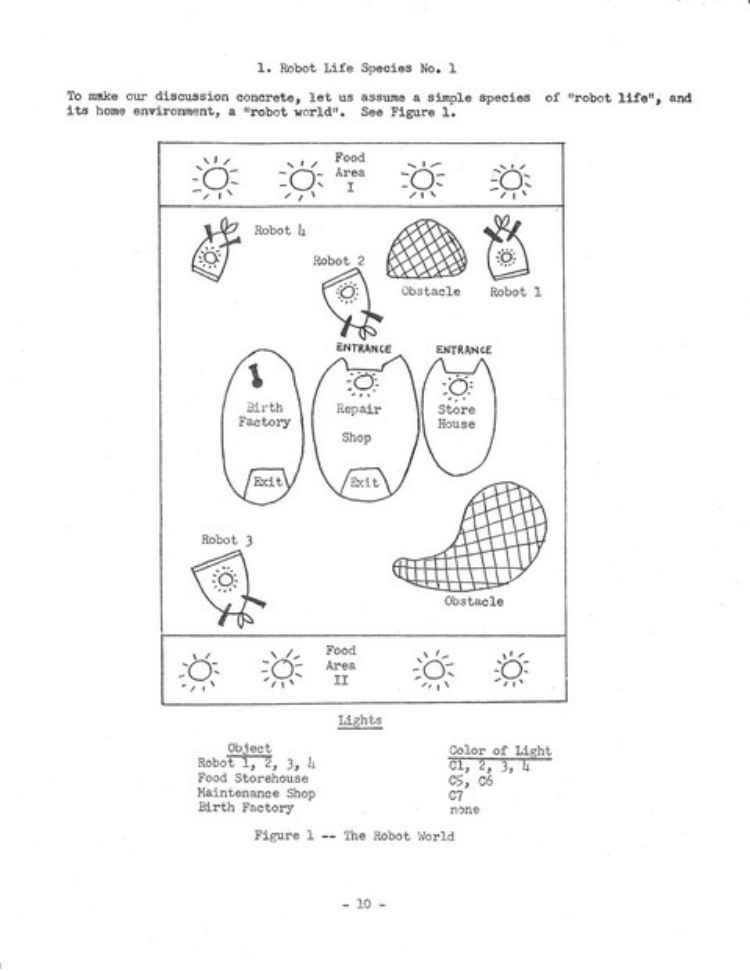
\includegraphics[width=\textwidth]{figures/page-13.png}
\caption{Figure 1 from the source volume, introducing ``Robot Life Species
No.\ 1'' and the robot world.}
\end{figure}

\begin{figure}[p]
\centering
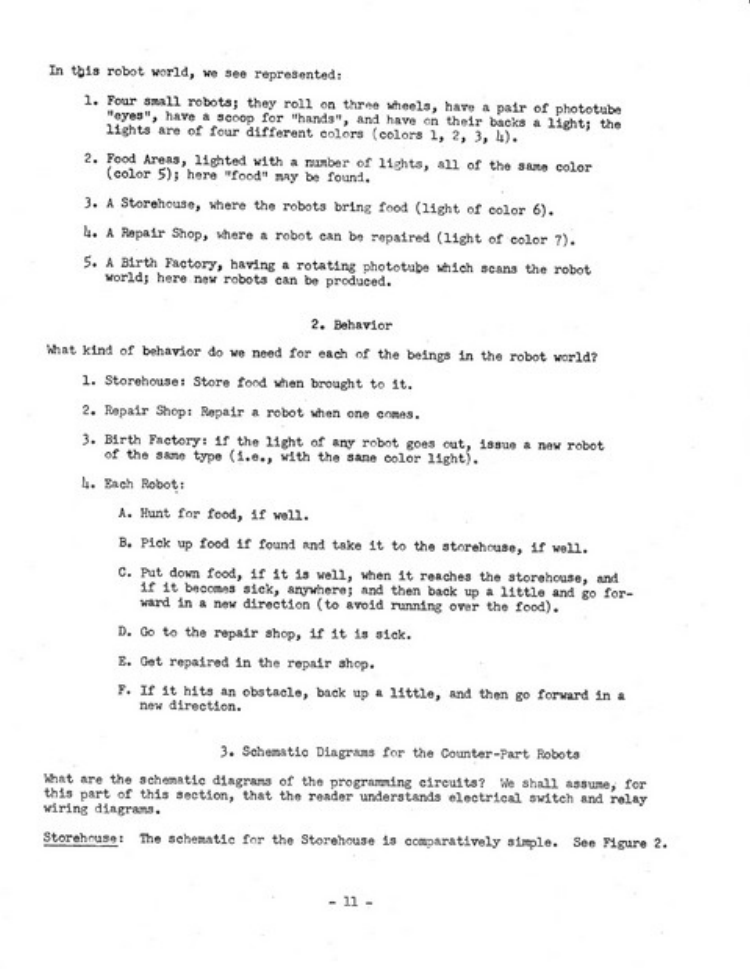
\includegraphics[width=\textwidth]{figures/page-14.png}
\caption{Source page continuing the description of Figure 1 and introducing the
textual lead-in to Figure 2.}
\end{figure}

\begin{figure}[p]
\centering
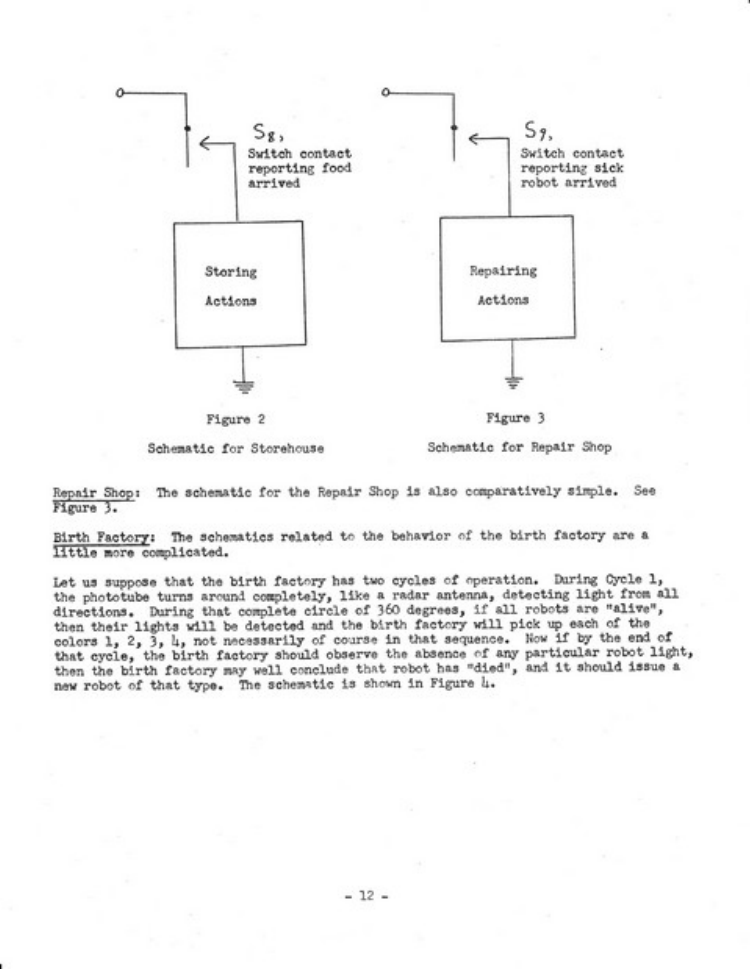
\includegraphics[width=\textwidth]{figures/page-15.png}
\caption{Figures 2 and 3 from the source volume: schematic diagrams for the
storehouse and repair shop.}
\end{figure}

\begin{figure}[p]
\centering
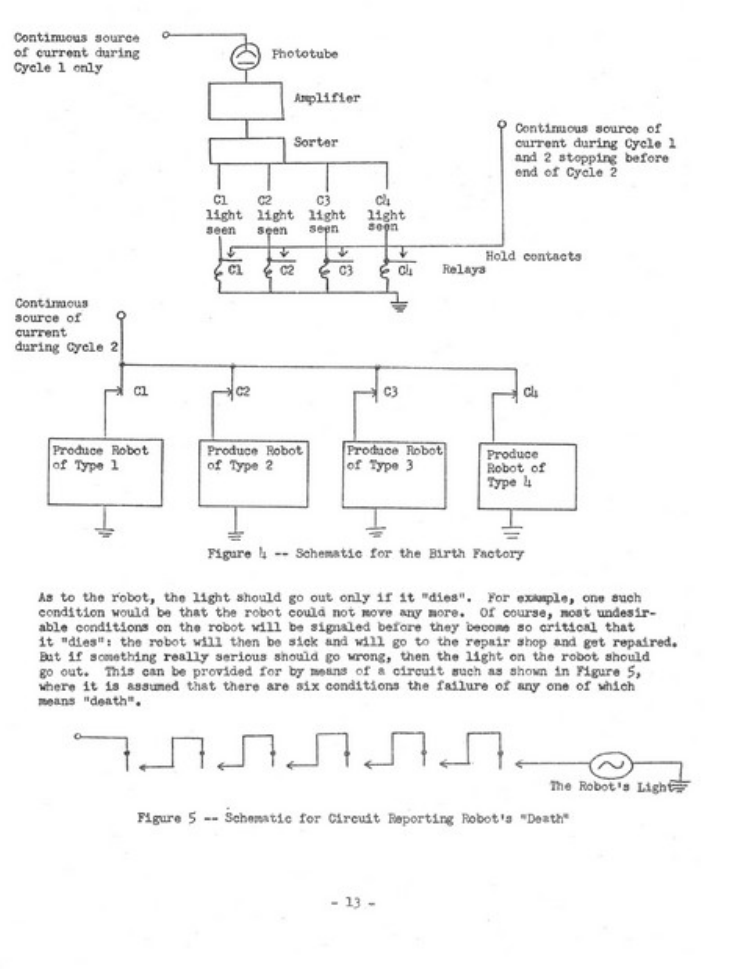
\includegraphics[width=\textwidth]{figures/page-16.png}
\caption{Figures 4 and 5 from the source volume: schematics for the birth
factory and for the circuit reporting a robot's ``death.''}
\end{figure}

\subsection*{4. Schematic Diagrams for the Robots}

We come now to the schematic diagrams for the behavior of any of the four
robots.

First, the needed senses of the robot are these:

\begin{tabularx}{0.96\textwidth}{@{}r Y >{\RaggedLeft\arraybackslash}p{0.08\textwidth}@{}}
No. & Sense & Relay \\
1 & See light with its left eye & $S_1$ \\
2 & See light with its right eye & $S_2$ \\
3 & Detect the light of the food (color 5) & $S_3$ \\
4 & Detect the light of the storehouse (color 6) & $S_4$ \\
5 & Detect the light of the repair shop (color 7) & $S_5$ \\
6 & Detect the presence of food in its scoop & $S_6$ \\
7 & Detect an obstacle & $S_7$ \\
8 & Detect the entrance of the storehouse & $S_8$ \\
9 & Detect the entrance of the repair shop & $S_9$ \\
10 & Realize that it has become sick & $S_{10}$ \\
11 & Realize that it has become well & $S_{11}$ \\
\end{tabularx}

In keeping with the outline nature of this report, we shall assume that these
senses may be contrived in hardware fairly easily and will result in the
picking up of relays, one for each sense. We should comment on the last two
senses, however, since they are essentially compound states. That is to say, if
there were, say, seven conditions such that the failure of any one of them
would mean ``sickness'', then there would be a circuit on the robot of the type
shown in Figure 6, picking up the $S_{10}$ relay that reports ``becoming
sick''.

Second, the needed actions of the robot will be: driving forward or backward,
or stopping; steering to the right or the left; or not steering; closing the
scoop; or opening the scoop. These actions it happens are the same as the
actions of Squee. So they may be contrived in hardware by referring to the
published plans for Squee. Also, converting the sight of the left and the right
eyes into adequate homing behavior --- ``phototropism'', like a moth to a
candle --- is a problem that has been solved and published for Squee.

Third, we need to consider the programming of the robot; by means of which it
will behave as we desire it to. This is a problem in the organization of
sequential relay circuits. But it can be quite easily handled and analyzed
using what we may call Boolean calculus, which is equal to Boolean algebra
extended by a new operator which provides for delay, i.e., changes in time,
``before'' and ``after'', states and events. We shall assume for the remaining
part of this section that the reader understands Boolean algebra and the
applications of Boolean algebra to relay wiring circuits. By way of review,
however, these key definitions are these:

\begin{tabularx}{0.96\textwidth}{@{}>{\RaggedRight\arraybackslash}p{0.30\textwidth} Y@{}}
$a$ (written next to a relay contact) & the condition that ``the relay contact is closed''; or, the truth value of this condition, equal to 1 if true and 0 if false \\
$a$ (written next to a relay coil) & the condition that ``the relay coil is energized''; or, the truth value of this condition \\
$a \vee b$ & $a$ or $b$ or both; or, $a$ plus $b$ minus ($a$ times $b$), if $a, b = 0, 1$ \\
$a \cdot b$ & both $a$ and $b$; or, $a$ times $b$ if $a, b = 0, 1$ \\
$a'$ & not $a$; or, $1$ minus $a$, if $a = 0, 1$ \\
$a^{+k}$ & the condition equal to $a$ but delayed $k$ units of time; or, if $a = f(t)$, then $a^{+k} = f(t+k)$ \\
\end{tabularx}

These variables may be thought of as time functions that have only the values 0
and 1, such as shown in Figure 7.

As an abbreviation for $a^{+1}$, we shall often use $\hat{a}$ or $a^{*}$.

Now suppose we want a relay to represent a state $S$ that continues during some
period. Suppose that that state $S$ starts with Event 1 and stops with Event 2.

The Boolean calculus equation will be:

\[
S = (E_1 \vee \hat{S}) \cdot E_2'
\]

The relay hold contact marked $\hat{S}$ has to lag slightly behind the coil
$S$. We shall assume that the lag is one unit of time, or one pulse time.
Physically, for many relays, the lag is often about 1/20 of a second, and is
called the pick-up time.

For another example of a delay function, let us consider a time delay relay.
This has the property that it energizes, say, five seconds after the contact
closes that leads to it; see Figure 8.

Here the Boolean calculus equation will be $B = A^{+100}$ or if we use seconds
as units of time, $B = A^{+5}$.

We are now ready to display the organization of the states, events, and
programming of our species of robot life. They are shown in Figure 9.

\begin{figure}[p]
\centering
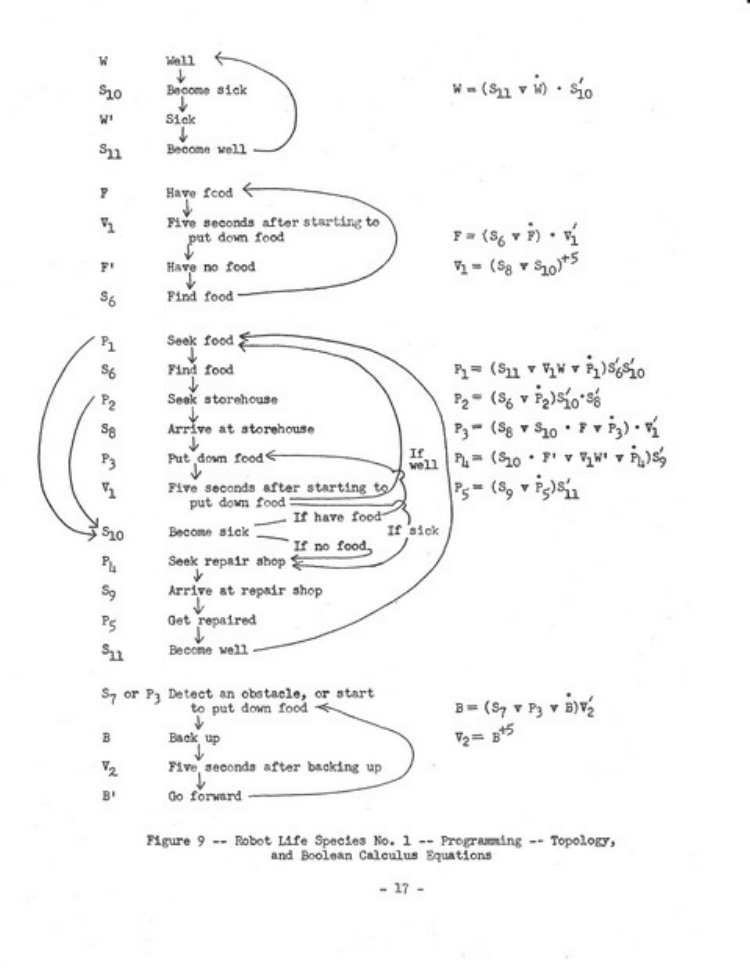
\includegraphics[width=\textwidth]{figures/page-20.png}
\caption{Figure 9 from the source volume: robot-life programming topology and
Boolean-calculus equations.}
\end{figure}

\begin{figure}[p]
\centering
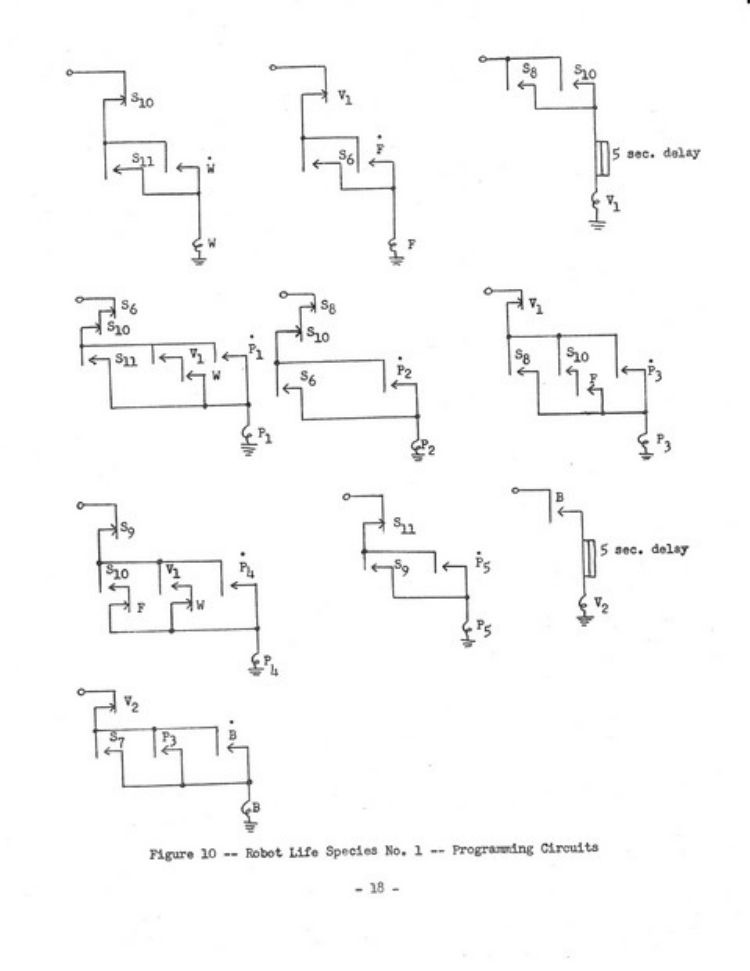
\includegraphics[width=\textwidth]{figures/page-21.png}
\caption{Figure 10 from the source volume: programming circuits for Robot Life
Species No.\ 1.}
\end{figure}

\clearpage

\section*{Part III --- Practical Conclusions}

Now is all this theoretical? What use is it? Who in the world wants living
robots anyhow?

Well, we do. In our small organization we are engaged in a small-scale program
of constructing brains and robots. We have finished Simon, a miniature
mechanical brain, and Squee, the robot squirrel; and we are at work on other
robots. We have in mind the construction of still other robots --- kinds that
will handle ideas, or live, or be companionable. Why do all this? It is
exciting to push back the frontier; it is fun to fire people's imagination; and
it seems to be good business.

But entirely apart from the interests of our own small organization, there is
no doubt that robots which are able to preserve themselves, repair themselves,
and reproduce themselves, will, as slaves or colleagues of men, open up
unheard-of, unimagined ways for human beings to pursue their goals.

For example, think of exploring the bottom of the ocean, or the interior of
volcanoes, or the surface of the moon, or the surface of Mars, with a swarm of
such robots. Think of dealing with plagues of caterpillars or locusts by hordes
of small flying robots about two inches long, equipped to slaughter such
insects. They would be much more economical and versatile than robots that
could not preserve or repair or reproduce themselves. In fact, it is not beyond
possibility that such robots already exist in present-day atomic energy or
guided missile installations, hidden in unscientific secrecy. In fact, in a
number of environments hostile or impossible for human beings or protoplasm
life, living robots will in the future become useful, practical, and essential.

\end{document}
